124. \begin{figure}[ht!]
\center{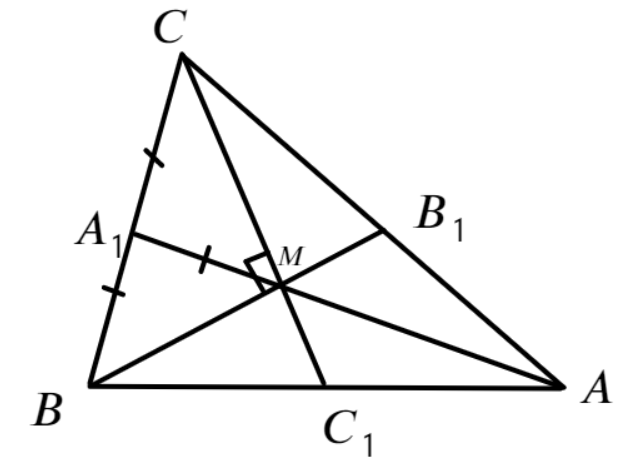
\includegraphics[scale=0.35]{g8-185.png}}
\end{figure}\\
Пусть медианы $BB_1$ и $CC_1$ пересекаются в точке $M.$ Тогда медиана $AA_1$ также проходит через эту точку и делится ей в отношении $2:1,$ значит $MA_1=36:3=12$см. Треугольник $BMC$ является прямоугольным, а $MA_1$ --- это его медиана, проведённая из прямого угла, значит она равна половине гипотенузы и $AC=2MA_1=24$см.\\
